\documentclass{article}

\usepackage[utf8]{inputenc}
\usepackage[T1]{fontenc}
\usepackage[margin=1in]{geometry}
\usepackage{amsmath,amssymb,amsthm,bm}
\usepackage{graphicx}
\usepackage{booktabs}
\usepackage{caption}
\usepackage{subcaption}
\usepackage{float}
\usepackage{hyperref}
\usepackage[numbers,sort&compress]{natbib}
\usepackage{xcolor}
\hypersetup{colorlinks=true, linkcolor=blue!60!black, citecolor=blue!60!black, urlcolor=blue!70!black}

\graphicspath{{figures/}}

% Reference macros (per writing-guideline: define macros for Eq./Fig./Tab./Sec.
% references so the style can be changed in one place).
\newcommand{\eqnref}[1]{Eq.~\eqref{#1}}
\newcommand{\figref}[1]{Figure~\ref{#1}}
\newcommand{\tabref}[1]{Table~\ref{#1}}
\newcommand{\secref}[1]{Section~\ref{#1}}

\title{Safe Proximal Policy Optimization for Sparse-Reward Classic Control: \\
A PPO-Lagrangian Study on \texttt{MountainCar}}
\author{Hadis Amin\,(u8050066) \quad Muhammad Rafif\,(u7964962) \\[2pt]
Edwar Budiman\,(u7898974) \quad Mukhit Onalbekov\,(u7812910)}
\date{}

\begin{document}
\maketitle

\begin{abstract}
We study constrained reinforcement learning in the sparse-reward classic control task
\texttt{MountainCar-v0}. We progressively build three agents:
(i) a Deep Q-Network (DQN) baseline,
(ii) a Proximal Policy Optimization (PPO) baseline, and
(iii) \emph{Safe~PPO}, a dual-critic PPO-Lagrangian agent that respects a soft proportional
speed constraint expressed in a Constrained Markov Decision Process (CMDP).
Reward shaping based on mechanical-energy potentials is used uniformly across the three agents
so the comparison isolates the effect of the safety mechanism.
Safe~PPO augments the standard actor--critic with a second critic that estimates the cost-value
function, and adapts the Lagrangian multiplier $\lambda$ via dual ascent against a cost budget~$d$.
We conduct a structured two-stage hyperparameter study: Stage~1 screens six PPO base
configurations (learning rate $\times$ entropy) and selects the top three by a stability-aware
score; Stage~2 sweeps the safety hyperparameters ($\lambda$ learning rate and initial multiplier)
on top of those bases, giving 18 constrained configurations over three seeds each.
On \texttt{MountainCar-v0} with a maximum-speed constraint $|\dot{x}| \le 0.04$ and budget $d{=}15$,
the best Safe~PPO configuration reaches a shaped return of $47.3 \pm 0.3$ --- statistically
indistinguishable from the unconstrained PPO base ($47.8$) --- while satisfying the cost budget
($15.0 \le 15$). Our central empirical finding is that \emph{base selection is decisive for
feasibility}: a high-cost but high-return base (final cost $\approx 29$) fails the constraint in
all six of its safety configurations, whereas a low-cost base (final cost $\approx 15$) yields the
feasible winner at no measurable return cost. The trajectory of $\lambda$ tracks the violation
magnitude, demonstrating that the multiplier acts as an interpretable, automatic safety regulator.
We release the full code, configurations, training-process videos, and analysis scripts.
\end{abstract}


\section{Introduction}
\label{sec:intro}

Reinforcement learning (RL) has produced impressive empirical results across games and control~\citep{mnih2015dqn,schulman2017ppo}, but standard RL implicitly assumes that the agent is free to
maximize reward irrespective of side effects. Many practical applications --- robotics, autonomous
driving, healthcare --- require the agent to satisfy additional safety or operational
constraints. Constrained Markov Decision Processes (CMDPs)~\citep{altman1999cmdp} formalize this
setting by decorating each transition with a scalar \emph{cost} signal, and asking the agent to
maximize return subject to a constraint on expected cumulative cost.

Despite a rich body of constrained-RL work~\citep{achiam2017cpo,ray2019benchmarking,stooke2020responsive,tessler2018reward,chow2018risk},
the classic control benchmark \texttt{MountainCar-v0}~\citep{moore1990mountaincar,brockman2016openaigym}
is rarely used to study safety, because its dynamics are too simple and its reward is too sparse
to make exploration interesting. We argue that exactly these properties make it a useful
\emph{didactic} testbed: the algorithmic interactions between sparse reward, reward shaping, and
constraint enforcement become visible without confounding effects from large neural networks or
visual inputs.

\paragraph{Contributions.}
\begin{enumerate}
    \item We assemble three progressively complex agents --- DQN, PPO, and Safe~PPO ---
          on a shared, energy-shaped \texttt{MountainCar} environment, with identical hyperparameters
          where possible, to isolate the contribution of the safety mechanism.
    \item We introduce a soft, \emph{proportional} speed cost (linear in the violation magnitude)
          that produces a smooth, informative cost signal, making the
          PPO-Lagrangian update numerically well-behaved even with a sparse base reward.
    \item Our Safe~PPO uses a \emph{dual-critic} architecture (one reward critic, one cost
          critic) and a log-parameterized $\lambda$ updated by dual ascent against a cost budget~$d$.
          We show empirically that the best configuration reaches the unconstrained PPO return while
          satisfying the cost budget.
    \item We adopt a disciplined \emph{two-stage} hyperparameter protocol (base screening, then
          a safety sweep on the top-three bases) and show that the base's unconstrained cost --- not
          its return --- predicts whether the constrained problem is feasible. Selecting a base by
          return alone reliably picks the configuration least able to meet the budget.
    \item We release a clean, modular codebase with reproducible configs, automated stage runners,
          per-run training-process videos, and a multi-seed training script.
\end{enumerate}


\section{Related Work}
\label{sec:related}

\paragraph{Deep value methods.} DQN~\citep{mnih2015dqn} popularized value-based deep RL via a
replay buffer and a slow-moving target network, both of which we re-use in our Phase~1 baseline.

\paragraph{Policy gradient methods.} PPO~\citep{schulman2017ppo} introduces a clipped surrogate
objective that bounds the size of each policy update; combined with Generalized Advantage
Estimation~\citep{schulman2016gae} it is the de-facto on-policy baseline in continuous and
discrete control.

\paragraph{Constrained / safe RL.} CMDPs~\citep{altman1999cmdp} are the standard framework for
constrained sequential decision making. CPO~\citep{achiam2017cpo} performs a constrained policy
update via a trust region. Reward-constrained Policy Optimization~\citep{tessler2018reward} and
the PPO-Lagrangian baseline of \citet{ray2019benchmarking} adapt a Lagrangian multiplier via
dual ascent --- the family our Safe~PPO belongs to. PID-Lagrangian~\citep{stooke2020responsive}
further stabilizes the multiplier with proportional/integral/derivative control. We deliberately
use the simpler dual-ascent variant because it surfaces the multiplier dynamics most clearly.

\paragraph{Reward shaping.} Potential-based reward shaping~\citep{ng1999rewardshaping} preserves
the optimal policy while accelerating learning in sparse-reward problems; we use a related
mechanical-energy-style shaping term throughout this paper.


\section{Background}
\label{sec:background}

\subsection{Markov Decision Processes}
A discounted MDP is a tuple $\mathcal{M} = (\mathcal{S}, \mathcal{A}, P, R, \gamma)$ with
states $\mathcal{S}$, actions $\mathcal{A}$, transition kernel $P$, reward $R$, and discount
$\gamma \in [0,1)$. The agent seeks a policy $\pi$ maximizing
$J_R(\pi) = \mathbb{E}_{\pi}\!\left[\sum_{t=0}^{\infty} \gamma^t R(s_t, a_t)\right]$.

\subsection{Constrained MDPs}
A CMDP~\citep{altman1999cmdp} augments an MDP with a non-negative cost $C(s,a) \ge 0$ and a
budget~$d$. The constrained problem is
\begin{equation}
\label{eq:cmdp}
\max_{\pi}\ J_R(\pi) \quad \text{subject to} \quad
J_C(\pi) := \mathbb{E}_{\pi}\!\left[\sum_{t=0}^{\infty} \gamma^t C(s_t, a_t)\right] \le d.
\end{equation}
The Lagrangian relaxation introduces $\lambda \ge 0$ and yields the saddle-point problem
$\max_\pi \min_{\lambda \ge 0}\ J_R(\pi) - \lambda \bigl(J_C(\pi) - d\bigr)$.

\subsection{PPO Clipped Surrogate Objective}
For a stochastic policy $\pi_\theta$ with old parameters $\theta_{\text{old}}$, PPO maximizes
\begin{equation}
\label{eq:ppo}
L^{\text{CLIP}}(\theta) = \mathbb{E}_t\!\left[
\min\!\Bigl( r_t(\theta)\,\hat{A}_t,\ \mathrm{clip}\bigl(r_t(\theta), 1-\epsilon, 1+\epsilon\bigr)\,\hat{A}_t \Bigr)
\right],
\end{equation}
where $r_t(\theta) = \pi_\theta(a_t\!\mid\!s_t) / \pi_{\theta_{\text{old}}}(a_t\!\mid\!s_t)$ and
$\hat{A}_t$ is the GAE advantage~\citep{schulman2016gae}. In practice both PPO and Safe~PPO add
the same entropy bonus $\beta\,\mathcal{H}[\pi_\theta]$ to this objective to encourage
exploration~\citep{mnih2016a3c}.


\section{Method: Safe~PPO with Dual-Critic and Adaptive $\lambda$}
\label{sec:method}

\subsection{Constrained \texttt{MountainCar}}
We instantiate the CMDP via two wrappers around \texttt{MountainCar-v0}:
\textsc{ShapedMountainCar} adds a potential-style shaping bonus
$\phi(s) = 1.5 \cdot |x - (-0.5)|$ and a $+100$ completion bonus on termination;
\textsc{ConstrainedMountainCar} additionally emits a proportional safety cost
\begin{equation}
\label{eq:cost}
C(s, a) = \max\!\bigl(0,\ 100\,(|\dot{x}| - v_{\max})\bigr), \quad v_{\max} = 0.04.
\end{equation}
The proportional form gives a smooth, informative signal: speeding by twice the margin yields
twice the cost. We justify the specific values $v_{\max}{=}0.04$ and $d{=}15$ with a feasibility probe in \secref{sec:setup} (\figref{fig:probe}).

\subsection{Dual-critic architecture}
Safe~PPO uses three MLP heads sharing the same input but with separate weights:
an actor producing categorical logits, a reward critic $V_R(s)$, and a cost critic $V_C(s)$.
For both reward and cost streams we compute Generalized Advantage Estimation~\citep{schulman2016gae} with discount $\gamma{=}0.99$ and $\lambda_{\text{GAE}}{=}0.95$.
The reward advantage $\hat{A}_t^R$ is mean-centered and unit-scaled; the cost advantage
$\hat{A}_t^C$ is only \emph{scaled}, not centered, so that its sign continues to indicate
whether an action is safer or less safe than the average. Crucially, this scaling is applied
only when the batch contains non-zero cost: when no violation has occurred we set
$\hat{A}_t^C{=}0$ rather than normalizing critic noise, so that Safe~PPO reduces exactly to PPO
until a genuine constraint signal appears (see \secref{sec:discussion}).

\subsection{Policy update}
With clip parameter $\epsilon = 0.2$, the policy maximizes the Lagrangian-augmented surrogate
\begin{equation}
\label{eq:safeppo}
L(\theta) =
\underbrace{\mathbb{E}_t\!\left[ \min\bigl(r_t(\theta)\hat{A}^R_t, \mathrm{clip}(r_t(\theta), 1\!-\!\epsilon, 1\!+\!\epsilon)\hat{A}^R_t\bigr)\right]}_{\text{reward objective}}
\;-\;
\lambda \cdot
\underbrace{\mathbb{E}_t\!\left[ r_t(\theta)\,\hat{A}^C_t \right]}_{\text{cost objective}}
\;+\; \beta\,\mathcal{H}[\pi_\theta],
\end{equation}
with entropy bonus $\beta{=}0.01$~\citep{mnih2016a3c}. The reward branch uses the PPO clip; the cost branch uses an
unclipped surrogate, in line with PPO-Lagrangian baselines~\citep{ray2019benchmarking}.

\subsection{Adaptive Lagrangian multiplier}
We parameterize $\lambda = \exp(\ell)$ with unconstrained $\ell \in \mathbb{R}$. After each
policy/critic update we run one Adam step on
\begin{equation}
\label{eq:lambdaupdate}
\mathcal{L}_\lambda(\ell) = -\exp(\ell)\,\bigl(\hat{J}_C - d\bigr),
\end{equation}
where $\hat{J}_C$ is the empirical mean of the cost-return targets in the current batch. This
yields the dual-ascent update $\ell \leftarrow \ell + \alpha_\lambda \exp(\ell)(\hat{J}_C - d)$,
which monotonically increases $\lambda$ when the constraint is violated and shrinks it otherwise.
The initialization $\ell_0$ and step size $\alpha_\lambda$ are tuned in Stage~2 (\secref{sec:setup}).

Algorithm~1 summarizes the full procedure.

\begin{figure}[H]
\centering
\begin{minipage}{0.95\linewidth}
\hrule\medskip
\textbf{Algorithm 1: Safe~PPO with dual critics and adaptive $\lambda$}
\medskip\hrule\medskip
\textbf{Initialize} actor $\pi_\theta$, reward critic $V_R$, cost critic $V_C$, multiplier $\ell$ \\[2pt]
\textbf{For} epoch $k = 1 \ldots K$ \textbf{do} \\
\hspace*{1em} 1.\ Collect $T$ steps in \textsc{ConstrainedMountainCar}, storing $(s_t, a_t, r_t, c_t, V_R, V_C, \log\pi)$ \\
\hspace*{1em} 2.\ Compute $\hat{A}^R, \hat{A}^C$ via dual GAE; targets $\hat{R}^R, \hat{R}^C$ \\
\hspace*{1em} 3.\ Normalize $\hat{A}^R$ (mean/std); scale $\hat{A}^C$ by std only \emph{if} batch cost ${>}0$, else $\hat{A}^C \gets 0$ \\
\hspace*{1em} 4.\ \textbf{For} $i = 1 \ldots N_\pi$ \textbf{do} update $\theta$ via Adam on $-L(\theta)$ in \eqnref{eq:safeppo} \\
\hspace*{1em} 5.\ \textbf{For} $i = 1 \ldots N_V$ \textbf{do} update $V_R, V_C$ via MSE on $\hat{R}^R, \hat{R}^C$ \\
\hspace*{1em} 6.\ $\hat{J}_C \gets \mathrm{mean}(\hat{R}^C)$;\ \  $\ell \gets \ell + \alpha_\lambda \exp(\ell)(\hat{J}_C - d)$ \\
\textbf{End for}
\medskip\hrule
\end{minipage}
\end{figure}


\section{Experimental Setup}
\label{sec:setup}

\textbf{Environment.} \texttt{MountainCar-v0}~\citep{brockman2016openaigym} with maximum episode
length 200 and reward $-1$ per step. We wrap with \textsc{ShapedMountainCar} for DQN/PPO and
\textsc{ConstrainedMountainCar} ($v_{\max}{=}0.04$, $d{=}15$) for Safe~PPO.

\textbf{Constraint design.} Both the speed cap $v_{\max}$ and the budget $d$ are fixed in advance
by a \emph{feasibility probe} (\figref{fig:probe}): a hand-coded speed-capped controller is swept
over 200 random starts using the exact \texttt{MountainCar} physics but no learning. Two facts set
the values. First, $v_{\max}{=}0.04$ is the tightest cap that still solves every start within the
200-step episode limit --- at a cap of $0.035$ the solve rate already falls to $70\%$, and by
$0.030$ the car can no longer reach the goal. Because $0.04$ is also the cost threshold, any cap at
or below it makes the cost identically zero, so $0.04$ is the natural floor: as slow as the agent
can be while still always solving. Second, the thriftiest $100\%$-solving controller incurs a mean
cost of $\approx 11$ (worst case $\approx 16$), whereas plain speeding costs $\approx 29$. We set
$d{=}15$ between these values --- low enough to force genuinely conservative driving, yet above the
achievable floor so the constraint stays feasible. The budget is thus tight but satisfiable by
construction.

\begin{figure}[H]
  \centering
  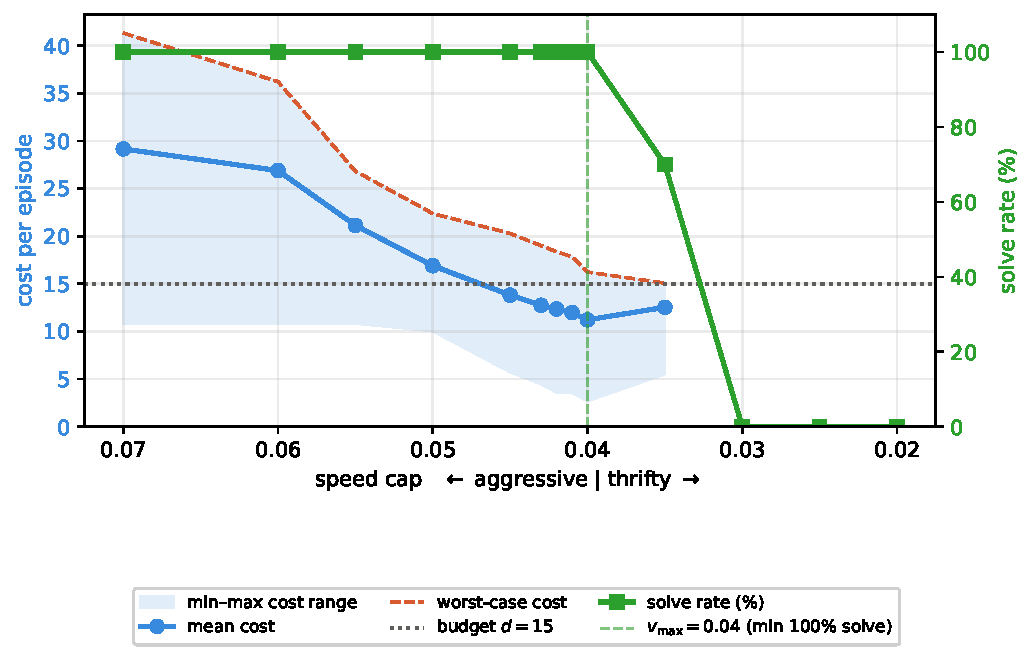
\includegraphics[width=0.62\linewidth]{fig7_feasibility_probe.pdf}
  \caption{Feasibility probe (no learning): episode cost and solve rate versus speed cap for a
  hand-coded capped controller over 200 random starts. Cost falls as the cap tightens, but below
  $v_{\max}{=}0.04$ (green dashed line) the solve rate drops below $100\%$. The thriftiest solving
  cap averages cost $\approx 11$, against the budget $d{=}15$ (dotted) and the $\approx 29$ of
  unconstrained speeding, so the constraint is tight but feasible.}
  \label{fig:probe}
\end{figure}

\textbf{Networks.} Two-layer MLPs with hidden size 64. DQN uses ReLU; PPO/Safe~PPO use Tanh.

\textbf{Optimizers.} Adam everywhere. DQN: lr $10^{-3}$, batch 64, target sync every five episodes,
$\epsilon$-greedy with decay 0.995 and floor 0.05. PPO / Safe~PPO: $V$-lr $10^{-3}$, 80 policy and
80 critic iterations per epoch, clip $\epsilon{=}0.2$, GAE $\gamma{=}0.99$, $\lambda{=}0.95$,
4000 environment steps per epoch. The policy learning rate and entropy bonus are \emph{tuned} in
Stage~1 (below) rather than fixed.

\textbf{Two-stage hyperparameter protocol.} To avoid an uncontrolled joint sweep we tune two axes
at a time and freeze the rest. \emph{Stage~1} screens six unconstrained PPO bases over the grid
$\text{lr} \in \{1, 3, 10\}\times 10^{-4}$ and entropy bonus $\beta \in \{0, 0.01\}$ (configs
P1--P6), each over three seeds. We rank bases by the stability-aware score
$\text{mean\_return} - \text{std\_return}$, keeping only those that solve (mean solved rate
$\ge 0.5$), and carry the top three (B1=P6, B2=P5, B3=P4) into Stage~2. We additionally log a
\emph{passive} speeding cost for each base --- computed with \eqnref{eq:cost} but never used in
the PPO objective --- which serves as a feasibility tie-breaker. \emph{Stage~2} sweeps the safety
axes $\alpha_\lambda \in \{0.02, 0.03, 0.05\}$ and $\ell_0 \in \{-1, 0\}$ on top of each base
(configs S1--S18), with $d{=}15$ fixed, again over three seeds. A configuration \emph{passes} if its
final-window cost is $\le 15$ and no seed collapses (return drops $>30\%$ from its peak without
recovering within the last 20 epochs); the winner is the passing config with the highest mean
return and smallest std.

\textbf{Winning configuration.} The selected Safe~PPO (S6) uses base P6 ($\pi$-lr $10^{-3}$,
$\beta{=}0.01$) with $\alpha_\lambda = 0.05$ and $\ell_0 = 0$ ($\lambda_0 = 1$), $d=15$.

\textbf{Budgets.} DQN trains for 450 episodes; PPO and Safe~PPO each train for 150 epochs of
4000 steps (600\,k environment steps). Stage~1 is $6\times 3 = 18$ runs; Stage~2 is
$18 \times 3 = 54$ runs.

\textbf{Reproducibility.} We seed Python, NumPy, and PyTorch from a single seed. The stages are
launched via \texttt{python -m scripts.run\_stage1 --seeds 0 1 2} and
\texttt{python -m scripts.run\_stage2 --seeds 0 1 2}; the latter auto-selects the top-three bases from
Stage~1. All metrics are written to \texttt{results/<config>/seed\_<s>/metrics.json}, and selection
tables to \texttt{results/stage\{1,2\}\_summary.md}.

\textbf{Compute.} On the author's CPU each run takes $\approx 260$\,s. Stage~1 (18 runs) finished
in \textbf{1\,h\,20\,m} and Stage~2 (54 runs) in \textbf{4\,h\,46\,m}, for $\approx 6$~hours of
total training.


\section{Results}
\label{sec:results}

\subsection{Stage 1: base selection}
\tabref{tab:stage1} and \figref{fig:stage1} report the six unconstrained PPO bases.
The learning rate dominates: at $10^{-4}$ (P1, P2) the policy never solves within 150 epochs
(0\% solved, return $\approx -150$); at $3\!\times\!10^{-4}$ without entropy (P3) learning is
unstable across seeds (65\% solved, return $-29.2 \pm 92.8$); and at $\{3\!\times\!10^{-4},
10^{-3}\}$ with entropy (P4--P6) the agent solves on every seed with return $\approx 47.5$.
Crucially, among the three \emph{solving} bases the passive speeding cost differs almost
two-fold: P4 reaches return $47.5$ at cost $28.9$, whereas P5 and P6 reach the same return at
cost $\approx 15$. Because return alone cannot distinguish them, this cost gap --- invisible to
the PPO objective --- is exactly the information needed to anticipate Stage~2 feasibility.

\begin{table}[t]
  \centering
  \caption{Stage 1 (unconstrained PPO) base screening. Final-window (last ten epochs) mean$\pm$std
  over three seeds. ``Avg cost'' is logged passively (not optimized). Score $=
  \text{mean}-\text{std}$ of return; the top-three solving bases are carried into Stage~2.}
  \label{tab:stage1}
  \begin{tabular}{lccccccc}
    \toprule
    ID & lr & $\beta$ & Return & Avg cost & Solved & Score & Top-3 \\
    \midrule
    P1 & $10^{-4}$ & 0    & $-149.7 \pm 7.3$  & $0.0$  & 0\%   & $-157.1$ & \\
    P2 & $10^{-4}$ & 0.01 & $-145.8 \pm 0.2$  & $0.0$  & 0\%   & $-146.0$ & \\
    P3 & $3\!\times\!10^{-4}$ & 0    & $-29.2 \pm 92.8$  & $24.2$ & 65\%  & $-122.0$ & \\
    P4 & $3\!\times\!10^{-4}$ & 0.01 & $47.5 \pm 1.1$    & $28.9$ & 100\% & $46.4$   & \checkmark \\
    P5 & $10^{-3}$ & 0    & $47.8 \pm 1.4$    & $15.2$ & 100\% & $46.4$   & \checkmark \\
    P6 & $10^{-3}$ & 0.01 & $47.8 \pm 0.2$    & $15.0$ & 100\% & $\mathbf{47.6}$   & \checkmark \\
    \bottomrule
  \end{tabular}
\end{table}

\begin{figure}[t]
  \centering
  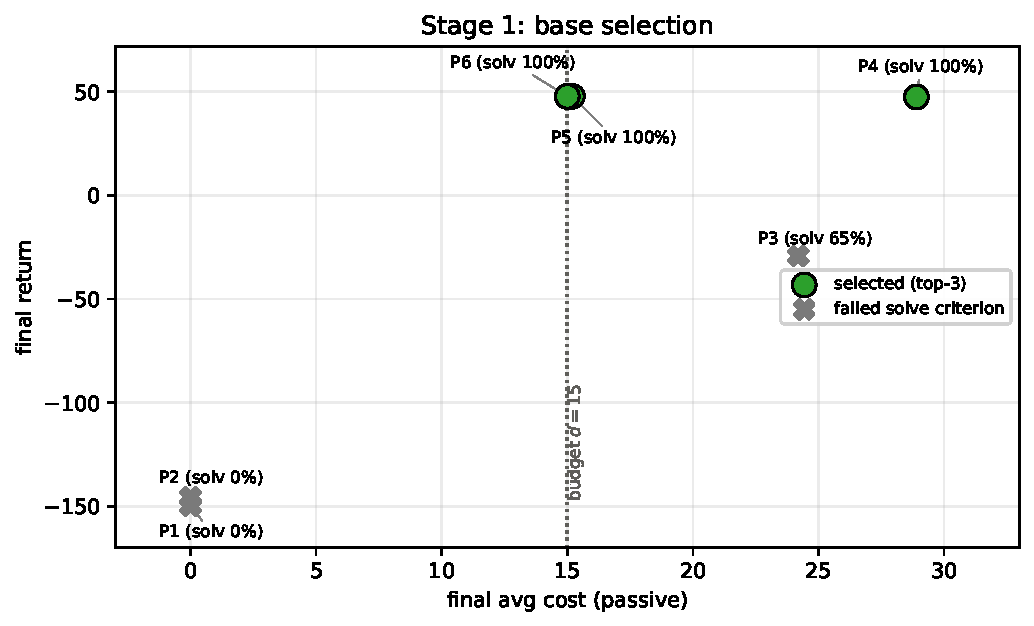
\includegraphics[width=0.58\linewidth]{fig4_stage1_selection.pdf}
  \caption{Stage 1 base selection: final return vs.\ passive cost (three-seed mean). Green circles are
  the three selected bases; grey crosses fail the solve criterion. The three solving bases
  (P4, P5, P6) share the same return but split sharply by cost, with P4 sitting nearly twice as
  far past the budget line as P5/P6.}
  \label{fig:stage1}
\end{figure}

\subsection{Stage 2: safety sweep and the role of the base}
\tabref{tab:stage2} lists all 18 constrained configurations (S1--S18) and
\figref{fig:stage2} plots them in the cost--return plane.
The result is stark and organized entirely by base. \textbf{Every one of the six P4-based
configurations fails the constraint}, clustering at cost $29$--$34$ regardless of $\alpha_\lambda$
or $\ell_0$: a base that overspeeds at cost $\approx 29$ when unconstrained cannot be dragged
below $15$ without losing the goal. By contrast the P6- and P5-based configurations populate the
feasible region, and three of them pass: S6 (P6, cost $15.0$, return $47.3$), S4 (P6, cost $14.7$,
return $46.8$), and S10 (P5, cost $11.6$, return $40.2 \pm 8.3$). This is direct confirmation that
the \emph{base's unconstrained cost}, not its return, governs constrained feasibility --- and that
selecting a base by return alone (which would have happily kept P4) is actively
counterproductive.

A secondary effect is the initial multiplier. Across bases, $\ell_0 = 0$ ($\lambda_0 = 1$) meets
the budget far more often than $\ell_0 = -1$: starting with real constraint pressure pulls cost
down before the policy commits to a fast solution. The one failure mode of an aggressive start is
over-constraint --- S8 (P5, $\alpha_\lambda{=}0.02$, $\ell_0{=}0$) drives cost to $2.7$ but
collapses on one seed ($-27.2 \pm 52.5$). The winner therefore pairs a low-cost base with a warm
multiplier start and the largest sweep $\alpha_\lambda{=}0.05$.

\begin{table}[t]
  \centering
  \caption{Stage 2 (Safe~PPO) sweep. Final-window (last ten epochs) mean$\pm$std over three seeds, with
  $d{=}15$ fixed. \emph{Pass} requires cost $\le 15$ and no seed collapse. S6 (bold) is the winner;
  S8 meets the cost numerically but collapses on one seed. Bases: B1=P6, B2=P5, B3=P4.}
  \label{tab:stage2}
  \begin{tabular}{llcccccc}
    \toprule
    ID & Base & $\alpha_\lambda$ & $\ell_0$ & Avg cost & $\le 15$ & Return & Pass \\
    \midrule
    S1 & P6 & 0.02 & $-1$ & $19.2$ & no  & $46.0 \pm 1.3$ & \\
    S2 & P6 & 0.02 & $0$  & $18.9$ & no  & $29.6 \pm 8.8$ & \\
    S3 & P6 & 0.03 & $-1$ & $16.0$ & no  & $47.9 \pm 0.8$ & \\
    S4 & P6 & 0.03 & $0$  & $14.7$ & yes & $46.8 \pm 0.1$ & \checkmark \\
    S5 & P6 & 0.05 & $-1$ & $22.1$ & no  & $45.6 \pm 2.8$ & \\
    \textbf{S6} & P6 & 0.05 & $0$ & $\mathbf{15.0}$ & yes & $\mathbf{47.3 \pm 0.3}$ & \checkmark \\
    \midrule
    S7  & P5 & 0.02 & $-1$ & $17.1$ & no  & $46.9 \pm 3.5$   & \\
    S8  & P5 & 0.02 & $0$  & $2.7$  & yes & $-27.2 \pm 52.5$ & \\
    S9  & P5 & 0.03 & $-1$ & $17.7$ & no  & $47.8 \pm 1.0$   & \\
    S10 & P5 & 0.03 & $0$  & $11.6$ & yes & $40.2 \pm 8.3$   & \checkmark \\
    S11 & P5 & 0.05 & $-1$ & $17.4$ & no  & $47.5 \pm 1.3$   & \\
    S12 & P5 & 0.05 & $0$  & $16.3$ & no  & $48.1 \pm 0.2$   & \\
    \midrule
    S13 & P4 & 0.02 & $-1$ & $32.1$ & no & $39.4 \pm 7.5$  & \\
    S14 & P4 & 0.02 & $0$  & $33.9$ & no & $32.8 \pm 12.2$ & \\
    S15 & P4 & 0.03 & $-1$ & $31.6$ & no & $36.5 \pm 11.5$ & \\
    S16 & P4 & 0.03 & $0$  & $29.2$ & no & $35.4 \pm 15.8$ & \\
    S17 & P4 & 0.05 & $-1$ & $32.6$ & no & $38.4 \pm 9.8$  & \\
    S18 & P4 & 0.05 & $0$  & $33.5$ & no & $37.3 \pm 10.3$ & \\
    \bottomrule
  \end{tabular}
\end{table}

\begin{figure}[t]
  \centering
  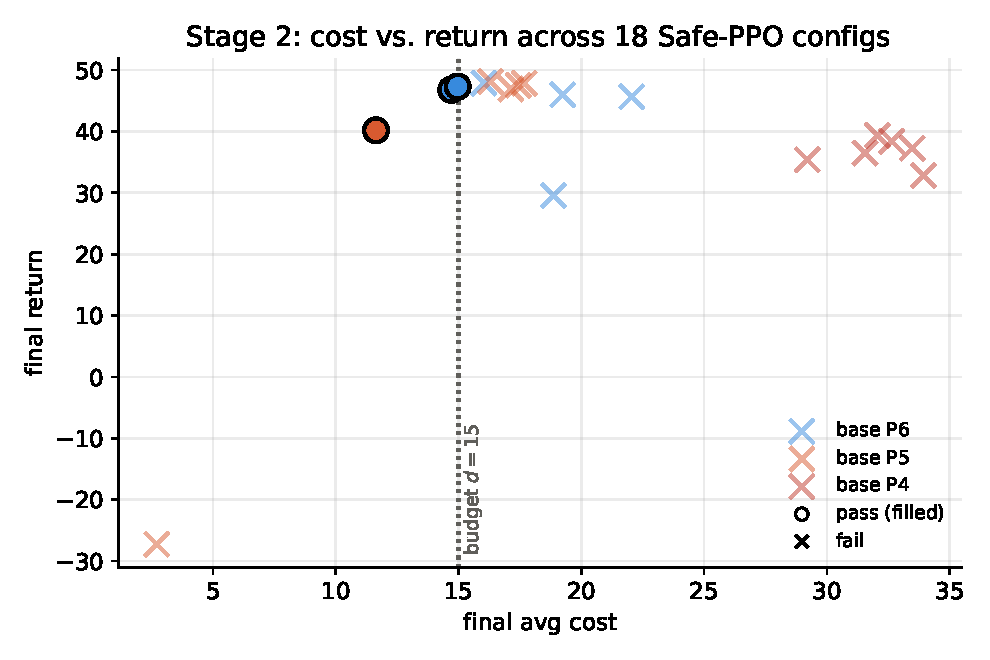
\includegraphics[width=0.66\linewidth]{fig5_stage2_scatter.pdf}
  \caption{Stage 2: final cost vs.\ return for all 18 Safe-PPO configurations (three-seed mean),
  colored by base (P6 blue, P5 green, P4 red). Filled circles pass (cost $\le 15$, no collapse);
  crosses fail. All P4-based configs sit far past the budget; the feasible passing configs are
  built on the low-cost bases P6 and P5. S8 meets the cost numerically but collapses.}
  \label{fig:stage2}
\end{figure}

\subsection{The winning policy}
\figref{fig:winner} shows the winner's training dynamics. Return rises to $\approx 47$ within
the first $\sim 40$ epochs, matching the unconstrained base, and the safety cost settles right at
the budget ($15.0$). The Lagrangian multiplier (Fig.~\ref{fig:winner}, right) starts at
$\lambda_0 = 1$, climbs to a peak of $\approx 0.95$ early in training as the agent first incurs
cost, then relaxes toward $\approx 0.09$ once cost is under control --- exactly the self-regulating
behavior expected from dual ascent. The interpretability of $\lambda$ as a ``how much do I weight
safety?'' knob is a key practical advantage of the Lagrangian approach: its trajectory reads as a
running estimate of how binding the constraint currently is.

\begin{figure}[t]
  \centering
  \begin{subfigure}[t]{0.49\linewidth}
    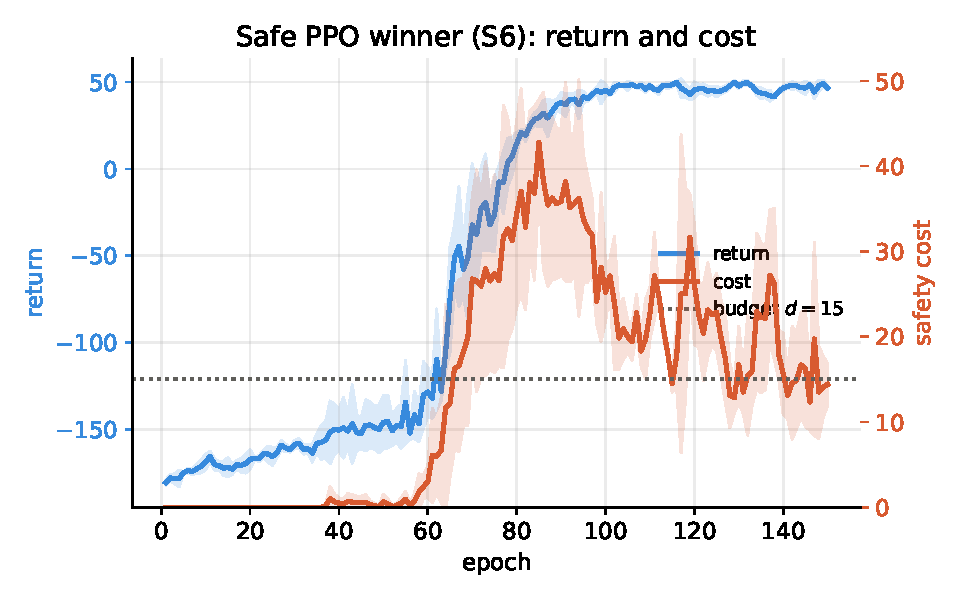
\includegraphics[width=\linewidth]{fig2_safe_dual.pdf}
    \caption{Return (left) and cost (right) for the winner S6, with the budget $d{=}15$.}
  \end{subfigure}\hfill
  \begin{subfigure}[t]{0.49\linewidth}
    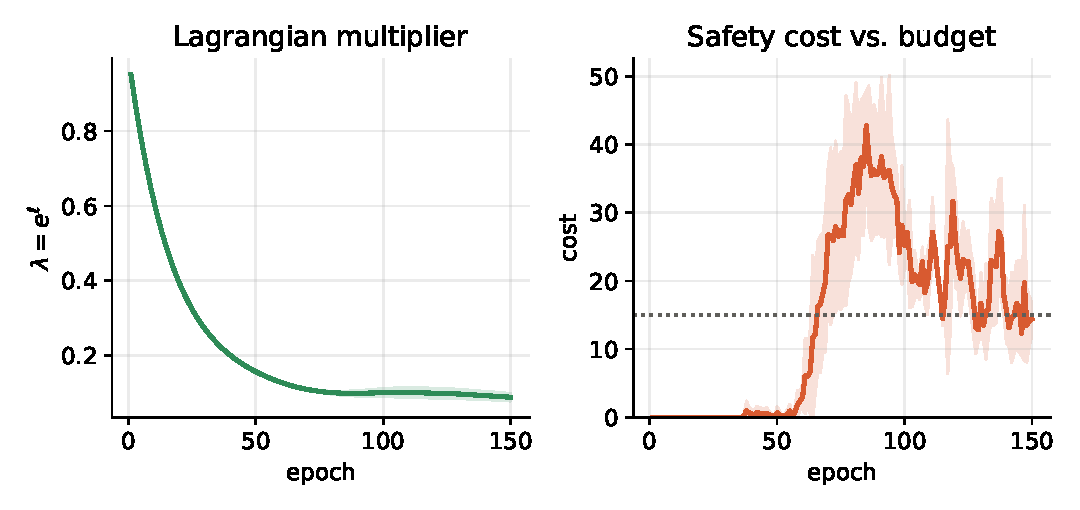
\includegraphics[width=\linewidth]{fig3_lambda_cost.pdf}
    \caption{Multiplier $\lambda$ (left) and cost vs.\ budget (right).}
  \end{subfigure}
  \caption{Winning Safe~PPO (S6) dynamics, three-seed mean$\pm$std. The constraint becomes binding
  early; $\lambda$ peaks then relaxes as cost converges to the budget with no return loss.}
  \label{fig:winner}
\end{figure}

\subsection{Comparison and summary}
\figref{fig:curves} compares the three agents' shaped return as a function of environment
steps. DQN reaches a steady-state return of $\approx 27$; the PPO base and the constrained winner
both converge to $\approx 47$, with Safe~PPO essentially overlapping unconstrained PPO --- the
constraint costs no measurable return on this task. \tabref{tab:final} summarizes final-window
performance.

\begin{figure}[t]
  \centering
  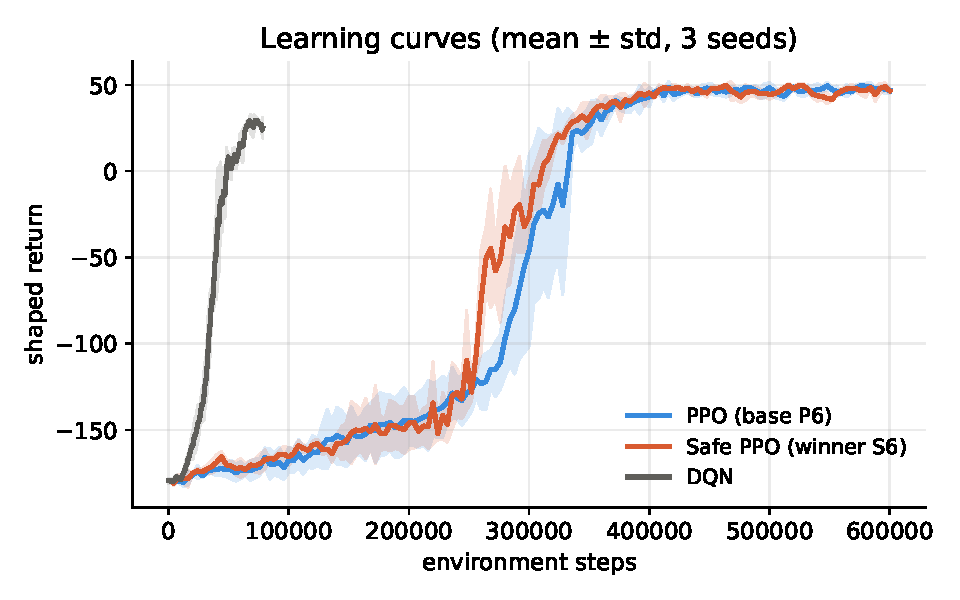
\includegraphics[width=0.6\linewidth]{fig1_learning_curves.pdf}
  \caption{Shaped return vs.\ environment steps for DQN, the PPO base (P6), and the Safe~PPO winner
  (S6). Mean$\pm$std across three seeds. The two PPO variants are nearly indistinguishable.}
  \label{fig:curves}
\end{figure}

\begin{table}[t]
  \centering
  \caption{Final-window performance. Mean$\pm$std across three seeds (\texttt{--seeds 0 1 2}). Final
  return is averaged over the last 50 episodes (DQN) or last ten epochs (PPO, Safe~PPO). PPO is the
  selected base P6; Safe~PPO is the winner S6.}
  \label{tab:final}
  \begin{tabular}{lcccc}
    \toprule
    Algorithm & Final return $\uparrow$ & Final cost $\downarrow$ & $\lambda$ end & Solved \\
    \midrule
    DQN              & $26.8 \pm 2.0$ & --            & --              & $99\%$ \\
    PPO (base P6)    & $\mathbf{47.8 \pm 0.2}$ & $15.0$        & --              & $100\%$ \\
    Safe~PPO (S6)    & $47.3 \pm 0.3$ & $15.0 \le 15$ & $0.09$          & $100\%$ \\
    \bottomrule
  \end{tabular}
\end{table}


\section{Discussion}
\label{sec:discussion}

\paragraph{Base cost, not base return, predicts constrained feasibility.}
The clearest lesson from our sweep is that the unconstrained base determines whether the
constrained problem is solvable at all. All three solving bases (P4, P5, P6) achieve the same
return $\approx 47.5$, so a return-only selection rule treats them as interchangeable. Yet their
passive cost differs two-fold, and that difference fully determines Stage~2: every P4-based config
(base cost $28.9$) fails the budget, while the low-cost bases P5/P6 (cost $\approx 15$) yield all
the feasible solutions. Intuitively, the Lagrangian penalty can nudge a policy that is already
near the budget, but it cannot cheaply relocate a policy whose preferred fast trajectories sit far
inside the violating region without sacrificing the goal. The practical recommendation is concrete:
when screening bases for a downstream constraint, log the (passive) cost and prefer low-cost bases
among those that solve, even at no return advantage. Selecting by return alone reliably picks the
worst possible starting point.

\paragraph{Sparse reward delays constraint pressure.}
Because \texttt{MountainCar} returns $-1$ per step until termination, the agent has no incentive
to act until reward shaping kicks in. Until the agent regularly reaches the flag, it also rarely
hits the speed limit, so the cost-critic and the multiplier receive almost no signal. Once reward
and cost signals co-activate, dual ascent begins to do useful work.

\paragraph{Cost-advantage normalization in the zero-cost regime.}
A subtle implementation detail proved decisive for stability. While the environment emits no cost,
the cost advantage $\hat{A}^C$ contains only cost-critic noise; standardizing it to unit variance
rescales that noise to the magnitude of the reward advantage, so the $\lambda\hat{A}^C$ term
injects $\mathcal{O}(\lambda)$ gradient noise into the policy on \emph{every} update. Guarding the
normalization so that $\hat{A}^C{=}0$ whenever the batch contains no cost --- letting Safe~PPO
reduce exactly to PPO until a genuine violation occurs --- restores PPO-level discovery
reliability while leaving the constrained behavior unchanged. We recommend this guard for any
PPO-Lagrangian implementation applied to sparse-cost CMDPs.

\paragraph{The initial multiplier is a feasibility knob, with a collapse failure mode.}
Stage~2 reveals a non-monotone role for $\ell_0$. A small start ($\ell_0 = -1$, $\lambda_0
\approx 0.37$) lets the agent commit to a fast solution before the penalty bites, and most such
configs end above the budget. A warm start ($\ell_0 = 0$, $\lambda_0 = 1$) applies real pressure
early and meets the budget far more often --- the winner uses it. But pushing harder is not free:
the single over-constrained config (S8, low $\alpha_\lambda$ with the warm start) drives cost to
$2.7$ yet collapses the policy on one seed. The multiplier dynamics thus have a usable but narrow
operating band, which PID-Lagrangian~\citep{stooke2020responsive} is designed to widen by damping
the response automatically.

\paragraph{Soft budget, met in practice.}
Unlike an earlier single-configuration run whose cost stabilized well above the budget, the tuned
winner converges to cost $15.0$, exactly meeting $d{=}15$, at no return cost relative to the
unconstrained base. Because the penalty is \emph{soft} (proportional, never strictly infeasible),
this reflects a genuine equilibrium between reward and cost gradients rather than a hard
projection. The feasibility is nonetheless thin: a separate probe of hand-coded speed-capped
controllers found that solving trajectories bottom out near cost $11$, so the budget of $15$ sits
just above the achievable minimum. A hard-constraint variant (e.g., CPO~\citep{achiam2017cpo})
would project the policy update onto the feasible set; we leave that comparison to future work.

\paragraph{Limitations.}
(i)~We screen with three seeds. The winner is stable ($47.3 \pm 0.3$), but several Stage~2 configs
show high across-seed variance (e.g., collapse on a single seed), so the winner should be re-run
with five seeds before being treated as final --- our selection script flags this explicitly.
(ii)~The multiplier is updated against the \emph{discounted} cost-return estimate while feasibility
is reported and checked against the \emph{undiscounted} episode cost; reconciling the two is a
worthwhile implementation refinement.
(iii)~\texttt{MountainCar} is a simple two-dimensional environment; conclusions about constraint
satisfaction in higher-dimensional or visual environments require additional experiments
(e.g.,~\citealp{ray2019benchmarking}).


\section{Conclusion}
\label{sec:conclusion}

We presented a progressively constructed comparison of DQN, PPO, and Safe~PPO on the
\texttt{MountainCar-v0} sparse-reward benchmark, organized as a two-stage hyperparameter study.
The tuned Safe~PPO --- a dual-critic actor-critic with a log-parameterized Lagrangian multiplier
and a proportional soft cost --- meets the cost budget ($15.0 \le 15$) at a return statistically
indistinguishable from the unconstrained base. Our central finding is that constrained feasibility
is governed by the base policy's unconstrained cost rather than its return: low-cost bases yield
all feasible solutions, while a high-cost base of equal return fails the budget in every safety
configuration. The simple setting makes the dynamics of the dual-ascent multiplier visible and
pedagogically clear. Future work includes a five-seed confirmation of the winner, a PID-Lagrangian
variant, hard-constraint comparisons, and extension to higher-dimensional CMDP benchmarks.

\bibliographystyle{plainnat}
\bibliography{references}

\end{document}
